\documentclass{article}
\usepackage{tikz, comment}
\usepackage{pifont}
\usepackage{fontspec, pgfplots}
\usetikzlibrary{arrows, decorations.markings, decorations.pathreplacing}
\begin{comment}
:Title: Not defined yet
:Tags: absolute value rules;properties of equality, equation rules;equivalence properties of equality;proper subset;element of a set
:Prob: 0.7838;0.7825;0.6701;0.667;0.6152
:Author: Prof.Hu Ji-shan, HKUST
:Slug: No name yet

Description Here.........
\end{comment}
\begin{document}\centering 

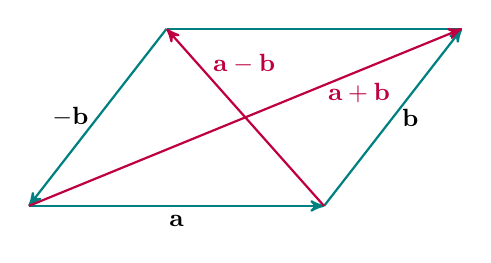
\begin{tikzpicture}[>=latex,xscale=.5*5, yscale=.5*5][font=\sf\small] 

%\draw[xstep=1cm,ystep=1cm,color=gray!80] (-1, -1) grid (4, 5);

\draw[teal, thick, ->, >=stealth'] (0,0)--(1.5, 0);
\node[below, scale=1] at ({1.5/2}, 0) {$\bf a$};

\draw[teal, thick, ->, >=stealth'] (1.5, 0)--(2.2, 0.9);
\node[right, scale=1] at ({(1.5+2.2)/2}, {0.9/2}) {$\bf b$};

\draw[teal, thick, >=stealth'] (2.2, 0.9)--(0.7, 0.9);


\draw[teal, thick, <-, >=stealth'] (0, 0)--(0.7, 0.9);
\node[left, scale=1] at (0.35, {0.9/2}) {$\bf -b$};

\draw[purple, thick, ->, >=stealth'] (0, 0)--(2.2, 0.9)node[below, midway, pos=0.75, xshift=2, yshift=0, scale=1]{${\bf a+b}$};

\draw[purple, thick, ->, >=stealth'] (1.5, 0)--(0.7, 0.9)node[right, midway, pos=0.8, xshift=2, yshift=0, scale=1]{${\bf a-b}$};

\end{tikzpicture}
\end{document}